\chapter{Methodology} \sloppy
\section{Software Development Approach}
 Agile is an iterative process-based approach to software development. In the Agile process model, work is broken down into more manageable, smaller iterations without requiring a lot of long-term planning. The requirements and scope of the project are determined early on, and the number, length, and scope of each iteration are preplanned. Each iteration is considered as a short time ``frame'' in the Agile process model, which lasts for a few weeks. In each iteration, teams move through the phases of the software development life cycle, which include planning, requirements analysis, design, coding, testing, and demonstration of a working product for client review. Agile places a significant value on flexibility, teamwork, and regular client feedback.\\
\begin{figure}[H]
    \centering
    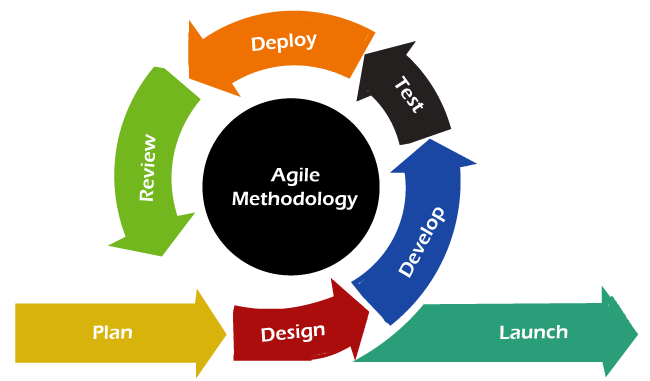
\includegraphics[width=80mm]{./img/agile.png}
    \caption*{\small{\textit{Source: https://www.javatpoint.com/agile-vs-waterfall-model}}}
    \caption{Agile Model}
\end{figure}
The main reason for which  we choose this development process:
\begin{enumerate}[noitemsep] %label=\Roman*.]
\item Very quick,flexible and efficient.
\item Risk minimization.
\item Projects are split into sprints for better management and productivity.
\item Through iterative testing and sprints, the final product contains less bugs. 
\item Development period for applications is reduced.
\end{enumerate}
\section{Data Collection} 
We will utilize the IStego100K dataset [7], a Large-scale open-source image steganalysis dataset. This dataset consists of a total of 200,000 images, serving as the primary resource for training and testing our model. Within the dataset, images are categorized into two main groups: ``Stego'' and ``Cover,'' each containing 100,000 images. The ``Stego'' subset contains images with hidden information added using three different methods. In contrast, the ``Cover'' subset consists of images without any hidden information added; they are in their original, unaltered state.\\
The size of images in the data set is 1024*1024 pixels.Each image in the dataset has randomly assigned quality factors in the range of 75-95. Three well-known steganographic algorithms J-uniward, nsF5, and UERD [8] [6] [7] are randomly selected for embedding in the images. The embedding rate for each image is randomly set in the
range of 0.1-0.4 bpac.
\section{Ensemble Classifiers}
Ensemble classifiers are machine learning techniques that combine multiple individual models, or ``base learners,'' to make predictions. Common ensemble techniques include bagging, boosting, and stacking. The main idea behind the ensemble methodology is to weigh several individual classifiers, and combine them in order to obtain a classifier that outperforms every one of them. A standard ensemble approach used in classification tasks consists of the following fundamental components:
\begin{enumerate}
    \item \textbf{Training set:} A labeled dataset is used for ensemble training. The instances of the dataset are described as attribute-value vectors. This set is crucial as it serves as the foundation for training the ensemble model, providing the necessary data points and their corresponding labels. In other words, it's the collection of data points used to train an ensemble learning algorithm. Each data point in the training set consists of two parts: the features (or attributes) and the label (or output). The features are the input variables used to predict the label, and the label is the output variable we want to predict.
    \item \textbf{Base Inducer:} The inducer is an induction algorithm that obtains a training set and forms a classifier that represents the generalized relationship between the input attributes and the target attribute. Decision trees, Neural networks, Support Vector Machines(SVMs), k-Nearest Neighbors(k-NN), Random Forsets, Gradient Boosting Machines(GBMs), (AdaBoost) etc. are different types of base learners that can be used in ensemble methods. The choice of base learner plays a vital role in the ensemble's performance and is often selected based on the nature of the problem and the characteristics of the data.
    \item \textbf{Diversity Generator:}This component is responsible for generating the diverse classifiers. Diversity among the classifiers is crucial as it helps improve the ensemble's performance by ensuring that the individual models provide different perspectives on the data. Techniques such as bagging, boosting, and randomization can be used to generate diverse classifiers.
    \item \textbf{Combiner:} The combiner is responsible for combining the classifications of the various classifiers. Some of the widely used combination methods are Weighting method, Majority voting, Performance weighting, Distribution summation, Bayesian combination, Dempster-Shafter, Vogging, Naive bayes. The choice of combination method depends on the nature of the problem and the characteristics of the data. The combiner's role is to aggregate the predictions of the individual models to produce the final ensemble prediction, which often leads to improved overall performance compared to using a single model.\cite{21} 
\end{enumerate}
\begin{figure}[H]
    \centering
    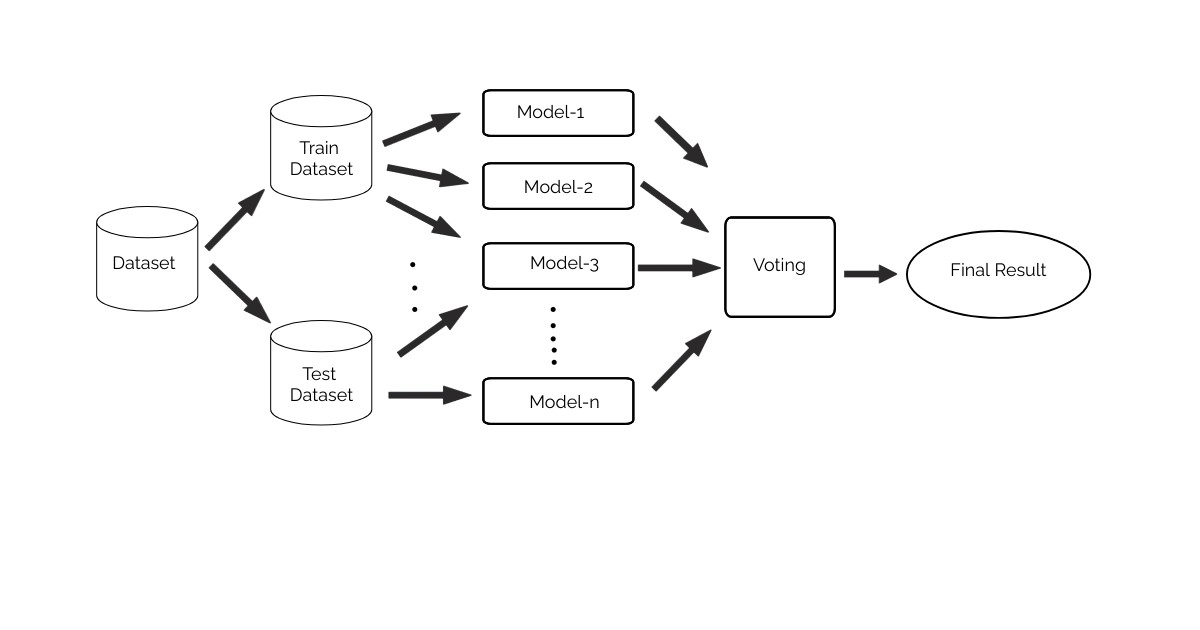
\includegraphics[width=160mm]{./img/ensemble.jpg}
    \caption{Basic outline of Ensemble Classifier}
\end{figure}

\subsection{Algorithm}
\begin{algorithm}
    \caption{Ensemble Classifier Algorithm \cite{5}}
    \begin{algorithmic}[1]
    \For{$l=1$ to $L$}
        \State Form a random subspace
        \State $D_l \subset \{1, \dots, d\}, \lvert D_l \rvert = d_{\text{sub}} < d$
        \State Form a bootstrap sample $N_1^b$, $\lvert N_1^b \rvert = N^{\text{trn}}$ by uniform sampling with \mbox{replacement} from the set $\{1, \dots, N^{\text{trn}}\}$
        \State Train a base learner $B_l$ on features
        \State $X_l = \{x_m^{(D_l)}, \bar{x}_m^{(D_l)}\}_{m \in N_l^b}$
        \State $\rightarrow$ obtain eigenvector $v_l$ and threshold $T_l$
    \EndFor
    \ForAll{$y \in Y^{\text{tst}}$}
        \For{$l=1$ to $L$}
            \State Make $l^{th}$ decision: $B_l(y^{D_l}) \triangleq \begin{cases} 1, & \text{when } v_l^Ty^{(D_l)} > T_l \\ 0, & \text{otherwise} \end{cases}$
        \EndFor
    \EndFor
    \State Form the final decisions $B(y)$ by majority voting: \\
    $B(y) = \begin{cases} 1, & \text{when } \sum_{l=1}^{L} B_l(y^{(D_l)}) > L/2 \\ 0, & \text{when } \sum_{l=1}^{L} B_l(y^{(D_l)}) < L/2 \end{cases}$
    \State \textbf{return} $B(y)$, $y \in Y^{\text{tst}}$
    \end{algorithmic}
    \end{algorithm}
    \clearpage
    \begin{flushleft}
    In the provided algorithm:\\
    \end{flushleft}
     $d$: Represents the dimensionality of the feature space.\\
     $d_{\text{sub}}$: Represents the dimensionality of the feature subset.\\
     $N^{\text{TRN}}$ and $N^{\text{TST}}$: Denote the number of training and testing examples, respectively.\\
     $L$: Represents the number of base learners.\\
     $x_m, \bar{x}_m \in \mathbb{R}^d, m=1,...,N^{\text{TRN}}$: Refer to the cover and stego features computed from the training set.\\
     $y_k, \bar{y}_k \in \mathbb{R}^d, k=1,...,N^{\text{TST}}$: Denote the cover and stego features computed from the testing set.\\

\section{Implementation}
CC-C300\cite{8} stands for Cardinal Cartesian - Co-occurrence. As the name suggests, ``Cardinal Cartesian'' refers to the use of coordinates. In this context, pixels and DCT values represent the coordinates. The use of these coordinates helps classify each pixel and its co-occurrence more precisely, but it comes at the cost of doubled dimensionality. The dimensionality is calculated as follows: CC-C300 utilizes the features of the top 300 important features, which are determined using the mutual information (MI) parameter. Each pixel provides a DCT value, further truncated by parameter T for more efficient co-occurrence matrix calculation between two different pixels. Consequently, each pixel results in an 81-dimensional output, and considering the co-occurrence between pixels, the total dimension becomes 2 * 81 * 300, which equals 48,600.
Due to its high dimensionality and the fact that our target model addresses the curse of Dimensionality (CoD), CC-C300 is the ideal feature to be extracted. Therefore, it is preferable to extract the CC-C300 feature for each .jpeg image out of 200k images. This extraction process should be conducted in batches of 10k for smoother and more efficient feature extraction.\vspace{0.2cm}
The ideal model to use for the aforementioned features is an ensemble classifier. An ensemble classifier is favored because it focuses more on diversity than accuracy in its base models. A high-accuracy base learner on a specific dataset may be less accurate when compared to a base learner with lower accuracy but a more diverse dataset. The model utilizes random "dsub," which selects random values from the image features during training. Out-of-Bag (OOB) is to be calculated based on the unused dataset while utilizing random bootstrapping.

\begin{figure}[H]
\section{Block diagram of proposed system}
 \centering
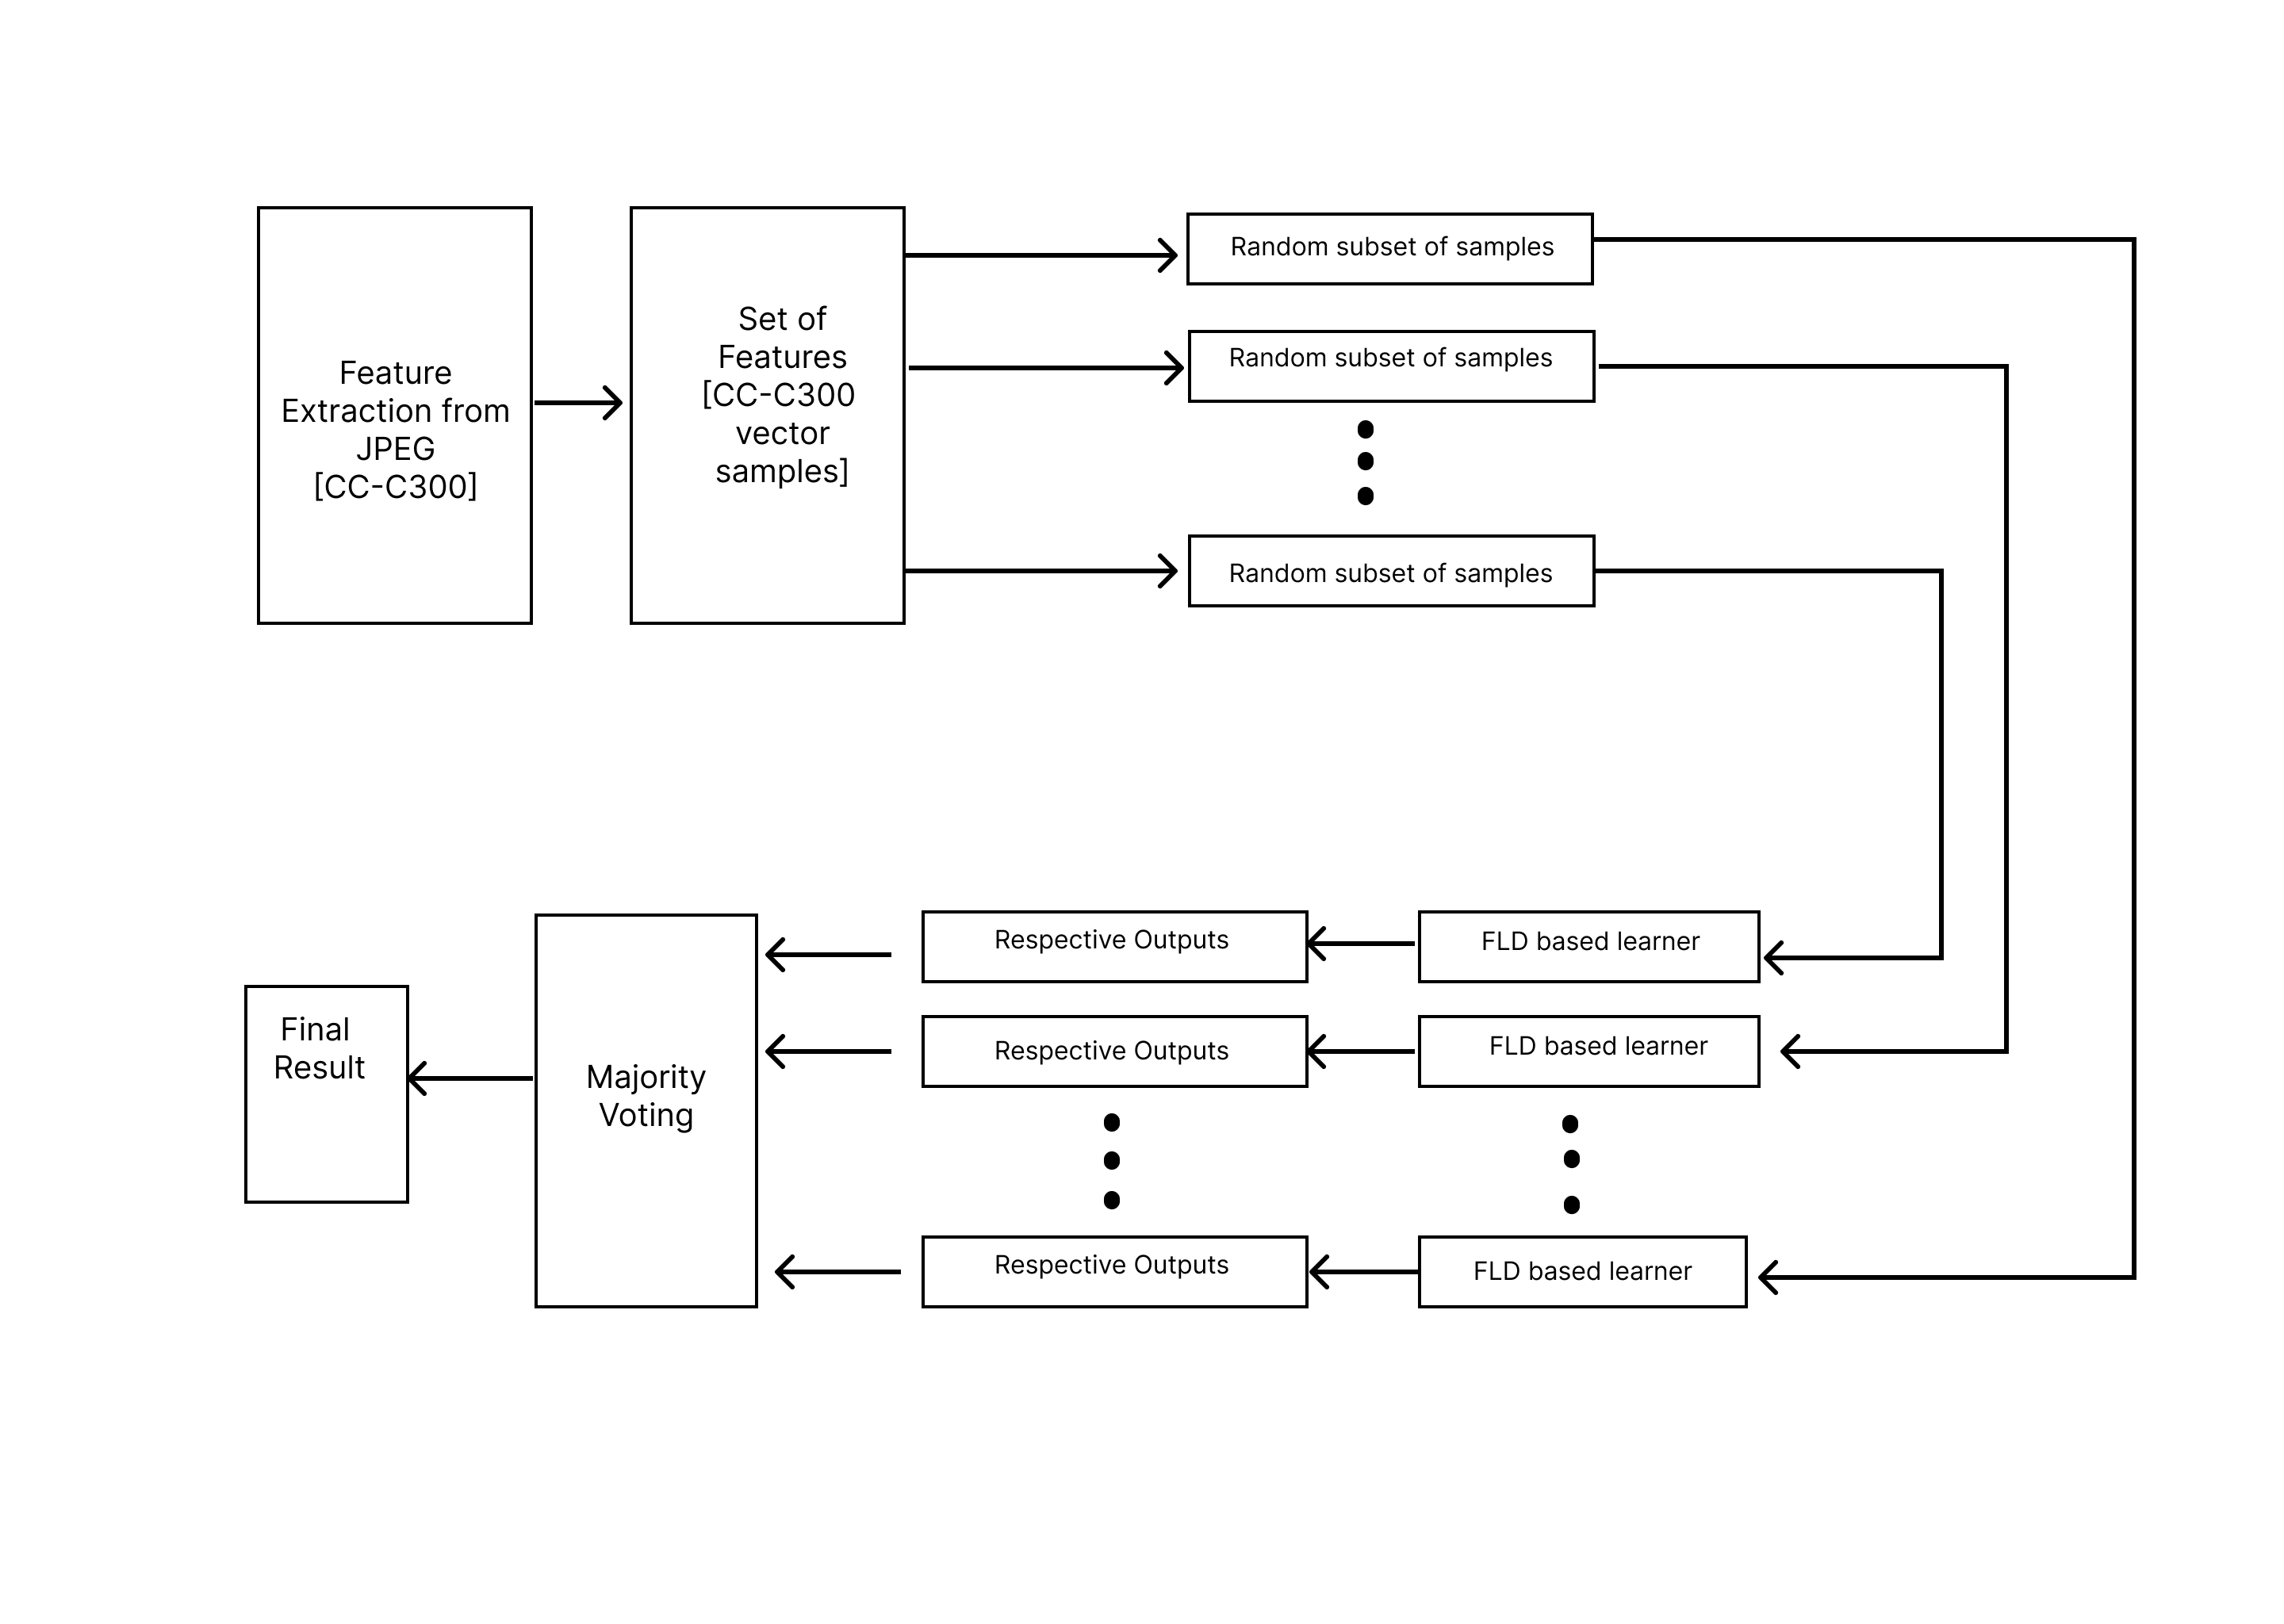
\includegraphics[width=140mm]{./img/model.png}\\
\caption{ Block diagram of proposed system}
\end{figure}
\clearpage

% \begin{flushleft}
%     \Large{\textbf{Model Training Approach}}\\
% \end{flushleft}
\section{Model Training Approach}
\textbf{Feature Extraction:}\\
CC-C300, denoting Cardinal Cartesian - Co-occurrence, employs coordinates derived from pixels and DCT values, enhancing precision in pixel classification and co-occurrence analysis. Despite the doubled dimensionality, the approach refines feature selection by utilizing the top 300 features determined through mutual information (MI). Each pixel contributes a DCT value, subsequently truncated by parameter T for efficient co-occurrence matrix computation. The resulting 81-dimensional output for each pixel contributes to an overall dimensionality of 48,600 (2 * 81 * 300). This strategic feature extraction methodology optimizes the representation of pixel relationships, combining the advantages of coordinate-based analysis and MI-based feature selection for robust image characterization.\vspace{0.25cm}\\
\textbf{Ensemble Classifier Selection:}\\
The decision for selecting an ensemble classification approach is based on the problem at hand. The bagging approach appears ideal for this classification problem as it effectively addresses issues such as overfitting, prevalent during model training. One of the main focuses of our model is diversity, and bagging achieves this by creating diverse bootstrapped samples, enhancing the accuracy of the classification. Bagging also allows parallelization, significantly reducing training time compared to other models like boosted ensemble classifiers, L-SVM, or G-SVM. The simplicity and instability of bagging contribute to its advantages for ensemble classification.\vspace{0.25cm}\\
\textbf{Bootstrapping:}\\
Bootstrapping is simply the process of randomly dividing the dataset into various parts and feeding them to the number of base learners present inside the ensemble classifier for training. The datasets are divided into various smaller samples and then sent to the base learners for training. This division of datasets removes their dependency on each other, promoting parallelization and allowing the training of various models simultaneously..\vspace{0.25cm}\\
\textbf{Base Learner Training:}\\
The base learners are fed with the feature "dsub," a subset of "d" where "d" is the total number of features or dimensions of each data. The base learners are trained on Fisher's Linear Discriminant Analysis (FLD), which outputs binary classification. FLD is chosen for its diversity in revealing various errors, increasing the diversity of each base learner and resulting in a more accurate ensemble classifier.\vspace{0.25cm}\\
\textbf{Aggregation:}\\
The trained model can now successfully classify the input images as cover or steganographically modified images. The binary classifier typically classifies 1 as a steganographically modified image and 0 as a cover image. The chosen voting method is hard voting, which calculates the number of 0s and 1s and outputs the result dominated by the majority. The threshold is set at L/2.
\vspace{0.25cm}\\
\textbf{Efficiency Considerations:}\\
The system prioritizes efficiency by embracing shallow machine learning techniques, specifically ensemble classifiers, instead of deep learning approaches. This strategic choice aligns with the computational efficiency goal, ensuring effective steganalysis without the computational demands associated with deep learning architectures. The intentional selection of CC-C300 as a feature further amplifies efficiency and bolsters the system's detection capabilities. This streamlined approach aims to strike a balance between accuracy and efficiency in steganalysis.\\

\section{System Architecture}
\begin{figure}[H]
    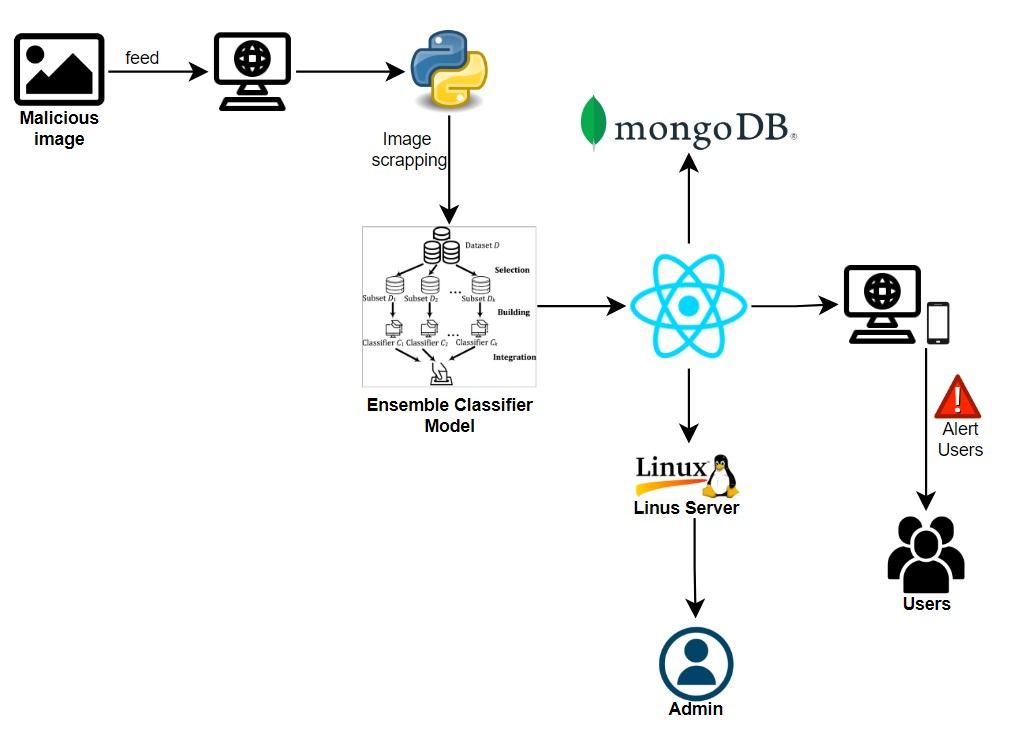
\includegraphics[width=150mm]{./img/System architecture.jpg}
    \caption{System Architecture}
\end{figure}
\clearpage 

